% Input this subsection under the Results section of report-8.tex.
% The parent document must load graphicx and set a path to this study's results/.
\subsection{Comprehensive Window Length Comparison}
\label{sec:comprehensive-window-length}

An earlier exploratory window experiment grouped session-holdout scores across sensor
combinations. It therefore did not isolate window length under
participant-independent testing. This follow-up varies window length alone
under a fixed Sydney-only XGBoost protocol. Its question is whether any length
between 20 and 240 seconds improves pooled held-out macro F1 over the
60-second setting used in the controlled transfer experiment.

\subsubsection{Cohort and feature construction}
The input is the frozen 166-session Sydney snapshot used by the controlled
study. Only bus, car, and train recordings with snapshot duration of at least
240 seconds are candidates; there is no upper-duration limit. After checking
the event data and requiring at least one quality-valid window at every one of
the 12 lengths, the common cohort contains 149 sessions from seven participants:
38 bus, 66 car, and 45 train. The same session identities and the same seven
participant folds are used at every length. The selection of longer,
quality-surviving sessions means that these estimates apply to a narrower set
than the main 60-second transfer evaluation.

Windows have lengths of 20, 40, \ldots, 240 seconds and advance by half their
length, giving 50\% overlap within a session. The Sydney feature pipeline
requires, for a window of length $W$ seconds, at least $30W$ accelerometer,
$4W$ gyroscope, and $2W$ magnetometer samples. A required sensor stream with a
consecutive-sample gap over 500 ms causes the window to be rejected. The fixed
11-feature vector contains mean, standard deviation, range, and minimum of
accelerometer and gyroscope magnitudes, plus standard deviation, range, and
minimum of magnetometer magnitude. Thus sensor inputs, feature definitions,
quality rules, and overlap fraction remain fixed while temporal context
changes.

\subsubsection{Training and evaluation}
For each length, the same leave-one-participant-out (LOPO) manifest holds out
one participant and trains on the other six. The fixed XGBoost parameters were
selected previously on NOR-TMD alone; this comparison trains each fold only
on Sydney windows, with class-balanced training weights and no NOR-TMD rows.
The three seeds are 42, 43, and 44. Twelve lengths by three seeds yield 36
completed evaluations and seven folds each, or 252 model fits. No held-out
participant contributes training windows in its fold.

Predictions from the seven held-out folds are pooled within each length and
seed. Macro F1 is the mean of bus, car, and train F1; balanced accuracy is the
mean of their recalls. Table~\ref{tab:comprehensive-window-grid} reports the
mean of the three seed-level pooled scores. Each session is tested once per
seed and length, but shorter lengths produce more overlapping windows. The
pooled metrics consequently weight sessions by their number of retained
windows and should not be read as participant-equal scores or as independent
journey counts.

The comparison against 60 seconds uses seed-matched macro F1 differences. To
describe uncertainty, 5,000 paired bootstrap draws resample the three seeds,
the seven participants, and sessions within sampled participants. Each draw
uses the same selections at the candidate length and at 60 seconds, then
recomputes pooled macro F1 from the sampled predictions. The displayed 95\%
intervals are the 2.5th and 97.5th percentiles of those differences. They
describe the recorded cohort and resampling scheme; they are not simultaneous
intervals adjusted for examining 11 alternatives to the baseline.

\subsubsection{Observed scores}
Figure~\ref{fig:comprehensive-window-curve} shows mean macro F1 rising from
0.596 at 20 seconds to 0.693 at 120 seconds, then fluctuating between 0.662
and 0.682 through 240 seconds. The 60-second reference scores 0.643. Balanced
accuracy follows a similar pattern, from 0.643 at 60 seconds to 0.691 at
120 seconds, but is omitted from the figure to keep the macro F1 trend clear.

\begin{figure}[htbp]
\centering
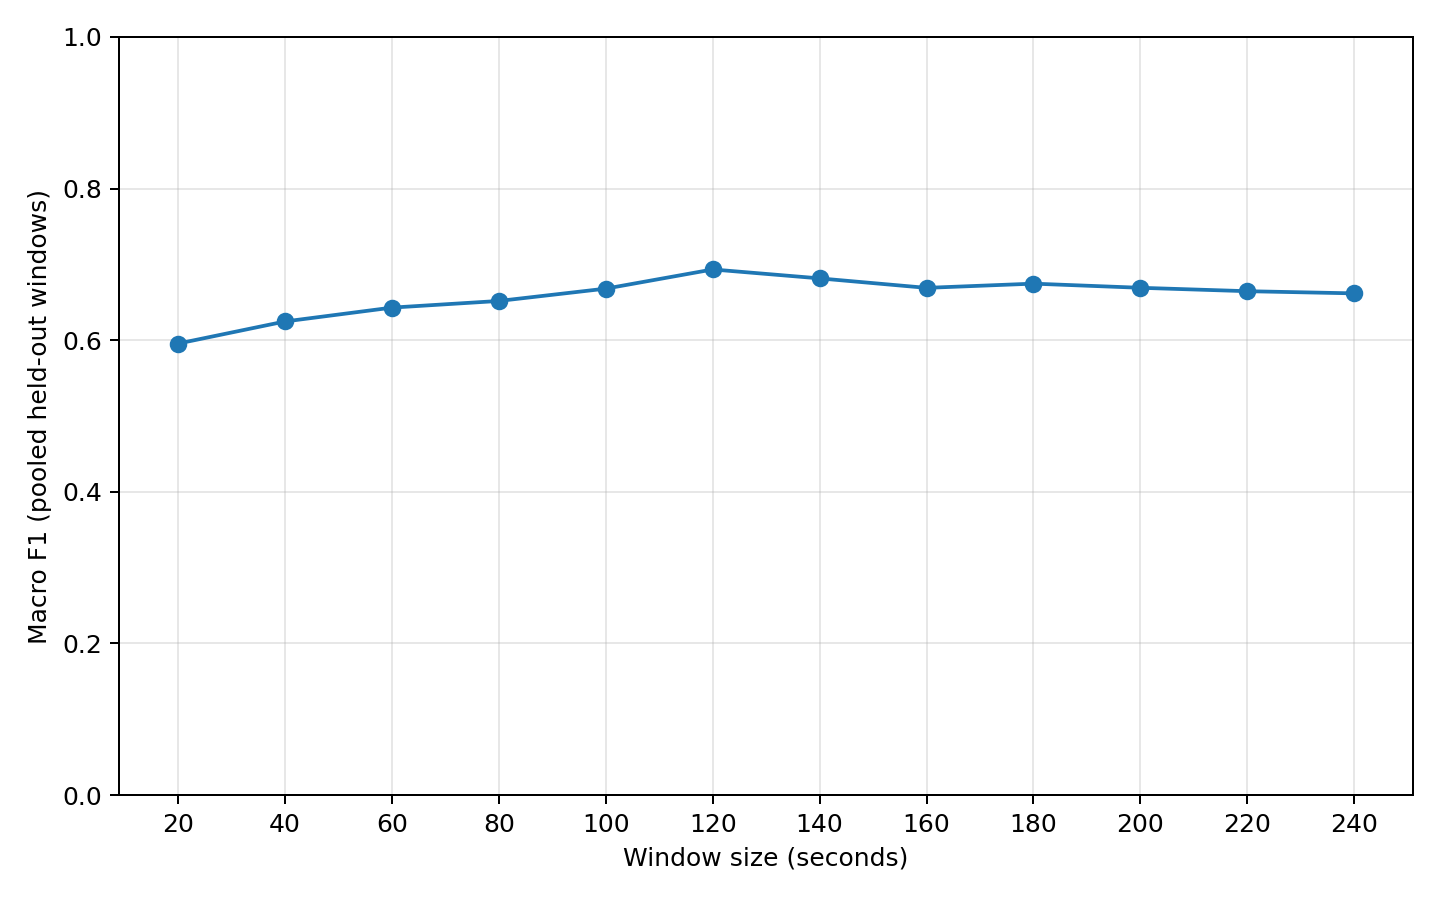
\includegraphics[width=0.88\linewidth]{window-curve.png}
\caption{Mean macro F1 on pooled held-out Sydney windows across three seeds.
The dashed vertical line marks the 60-second reference. All lengths use the
same 149 sessions, while the number of retained windows varies.}
\label{fig:comprehensive-window-curve}
\end{figure}

\begin{table}[htbp]
\centering
\small
\caption{Mean pooled scores across three seeds on the common 149-session
cohort. The final column is the seed-matched mean macro F1 difference from
60 seconds; Figure~\ref{fig:comprehensive-window-paired} gives its intervals.}
\label{tab:comprehensive-window-grid}
\begin{tabular}{rrrrr}
\hline
Window (s) & Mean windows & Macro F1 & Balanced accuracy & Difference \\
\hline
20  & 26,422 & 0.596 & 0.599 & $-0.047$ \\
40  & 13,099 & 0.625 & 0.626 & $-0.018$ \\
60  & 8,657  & 0.643 & 0.643 & $0.000$ \\
80  & 6,435  & 0.652 & 0.652 & $+0.009$ \\
100 & 5,107  & 0.668 & 0.666 & $+0.025$ \\
120 & 4,217  & 0.693 & 0.691 & $+0.050$ \\
140 & 3,580  & 0.682 & 0.679 & $+0.039$ \\
160 & 3,105  & 0.669 & 0.667 & $+0.026$ \\
180 & 2,733  & 0.675 & 0.673 & $+0.032$ \\
200 & 2,439  & 0.669 & 0.667 & $+0.026$ \\
220 & 2,196  & 0.665 & 0.663 & $+0.022$ \\
240 & 1,997  & 0.662 & 0.660 & $+0.019$ \\
\hline
\end{tabular}
\end{table}

The class-level pattern in Table~\ref{tab:comprehensive-window-classes}
helps explain the aggregate peak. From 60 to 120 seconds, bus F1 rises by
0.115, car F1 by 0.030, and train F1 by 0.006. Bus remains the most difficult
class at 120 seconds (F1 0.540), despite its larger gain. At 240 seconds,
train F1 has fallen to 0.664, while bus and car F1 remain above their
60-second values. These are descriptive changes on overlapping windows and
do not isolate a mechanism for the gains.

\begin{table}[htbp]
\centering
\small
\caption{Mean class F1 across the three seeds at selected window lengths.}
\label{tab:comprehensive-window-classes}
\begin{tabular}{rrrr}
\hline
Window (s) & Bus F1 & Car F1 & Train F1 \\
\hline
20  & 0.358 & 0.745 & 0.684 \\
60  & 0.426 & 0.788 & 0.715 \\
120 & 0.540 & 0.818 & 0.722 \\
240 & 0.513 & 0.808 & 0.664 \\
\hline
\end{tabular}
\end{table}

The largest positive point estimate against 60 seconds is at 120 seconds:
$+0.050$ macro F1, with a paired 95\% interval of $[-0.008,+0.087]$.
Figure~\ref{fig:comprehensive-window-paired} shows that this interval crosses
zero, as do those for the other longer windows. At 20 seconds, the estimate is
$-0.047$, with interval $[-0.079,-0.005]$; this is the only displayed
non-reference interval that excludes zero. The 120-second peak is therefore a
promising point estimate, while the paired analysis does not establish an
improvement over the 60-second reference.

\begin{figure}[htbp]
\centering
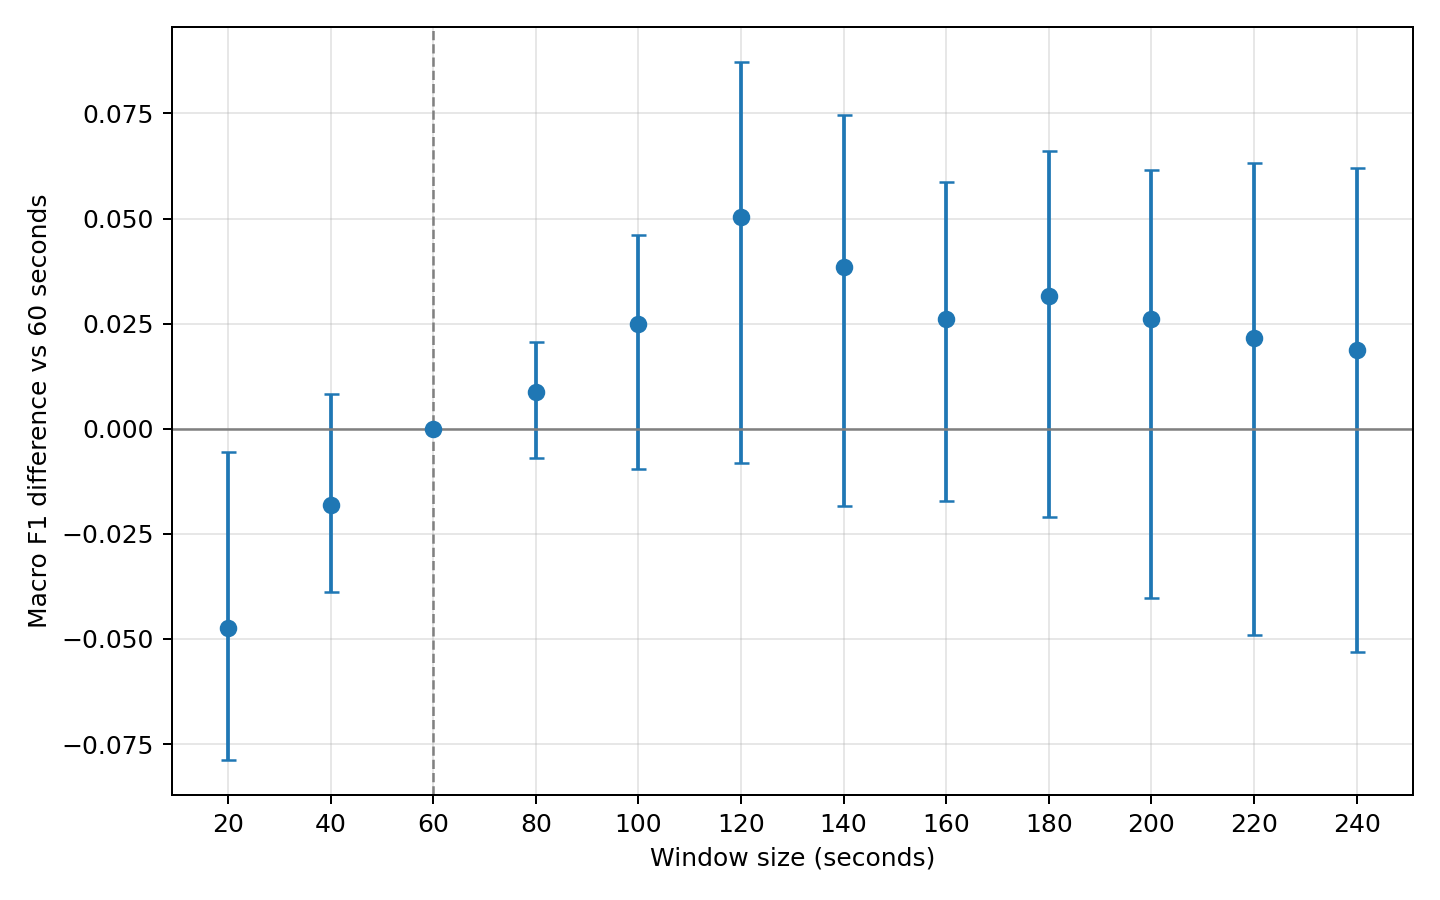
\includegraphics[width=0.88\linewidth]{paired-vs-60s.png}
\caption{Seed-matched mean macro F1 difference from 60 seconds. Error bars
show paired participant/session/seed bootstrap 95\% intervals. The horizontal
line is zero; the dashed vertical line marks the reference length.}
\label{fig:comprehensive-window-paired}
\end{figure}

\subsubsection{Relationship to the main evaluation}
The main controlled transfer evaluation uses 155 usable sessions and 8,668
windows at 60 seconds, yielding Sydney-only macro F1 of 0.648. This length
comparison uses the common 149-session cohort and 8,657 windows at 60 seconds,
yielding 0.643, because every included session must also support the
240-second condition. The two 60-second scores are therefore calculated on
different evaluation sets and should not be treated as repeated measurements
of identical test data. The feature definitions were informed by earlier
Sydney exploration, although the XGBoost parameters were selected on NOR-TMD
alone. This grid is a follow-up analysis rather than a prospective test of a
fully untouched design.

Longer windows provide more sensor history but fewer evaluation windows and a
longer wait for a first full-window prediction: nominally 120 seconds of
history and a 60-second update step at the observed peak. No on-device
latency, energy use, or transition-detection delay was measured. The seven
participants, class concentration, shared sessions across lengths, and
window-level pooling limit claims beyond this cohort. A new participant
cohort, ideally with the window length fixed in advance, is needed to check
whether the 120-second result persists.
